     The {\bf P}ortable {\bf U}niversity {\bf M}odel of the
     {\bf A}tmosphere {\bf (PUMA)} is based on the multi-level spectral
     model {\bf SGCM} ({\bf S}imple {\bf G}lobal {\bf C}irculation
     {\bf M}odel) described by \citep{hossim75} and \citep{jamesgray86}.
     Originally developed as a numerical prediction model,
     it was changed to perform as a circulation model. For example,
     \citep{jamesgray86} studied the influence of surface friction
     on the circulation of a baroclinic atmosphere, \citep{jamesjames92}
      and \citep{JamFraeJam94} investigated ultra-low-frequency
     variability, and \citep{molejames90} analyzed the baroclinic
     adjustment in the context of a zonally varying flow. \citep{frisius98}
      simulated an idealized storm track by embedding
     a dipole structure in a zonally symmetric forcing field and \citep{lunkeit98}
     investigated the sensitivity of GCM scenarios by using
     an adaption technique applicable to SGCMs.
     Storm track dynamics and low frequency variability
     was investigated by \citep{fraedrich2005}. For further citations search the
     bibliography at the end of this document and the list of publications at 
     {\url{http://www.mi.uni-hamburg.de/puma}}.

    
     PUMA was created with following aims in mind: training of junior
     scientists, compatibility with the {\bf ECHAM} 
     ({\bf E}uropean {\bf C}entre - {\bf HAM}burg) model and as a tool for
     further scientific investigations.
     

\section{Training of junior scientists and students}
     PUMA contains only the main processes necessary to simulate
     the atmosphere. The source code is short and clearly arranged.
     A student can learn to work with PUMA within a few weeks, whereas a
     full size GCM requires a team of specialists for maintenance,
     experiment design and diagnostics.
    
\section{Compatibility with other models}
     PUMA is designed to be compatible with other
     circulation models like Planet Simulator and ECHAM.
     The same triangular truncation is employed,
     and analogous transformation techniques like the Legendre- and
     Fast-Fourier transformation are used.
     The postprocessor {\bf Pumaburner} differs from ECHAM's
     {\bf Afterburner} only in respect to the format of the model's
     raw data which overcomes some problems of the ECHAM data format.
     PUMA uses a more compact though more precise
     format compared to the {\bf GRIB} ({\bf GRI}dded {\bf B}inary),
     which is used for ECHAM output.
     The Pumaburner supports the output formats SERVICE and
     NetCDF. All diagnostics and graphics software that are used with the
     ECHAM/Afterburner data can be used with PUMA/Pumaburner
     in exactly the same way.

\pagebreak
    
\begin{figure}
\centering
\begin{minipage}{0.75\linewidth}
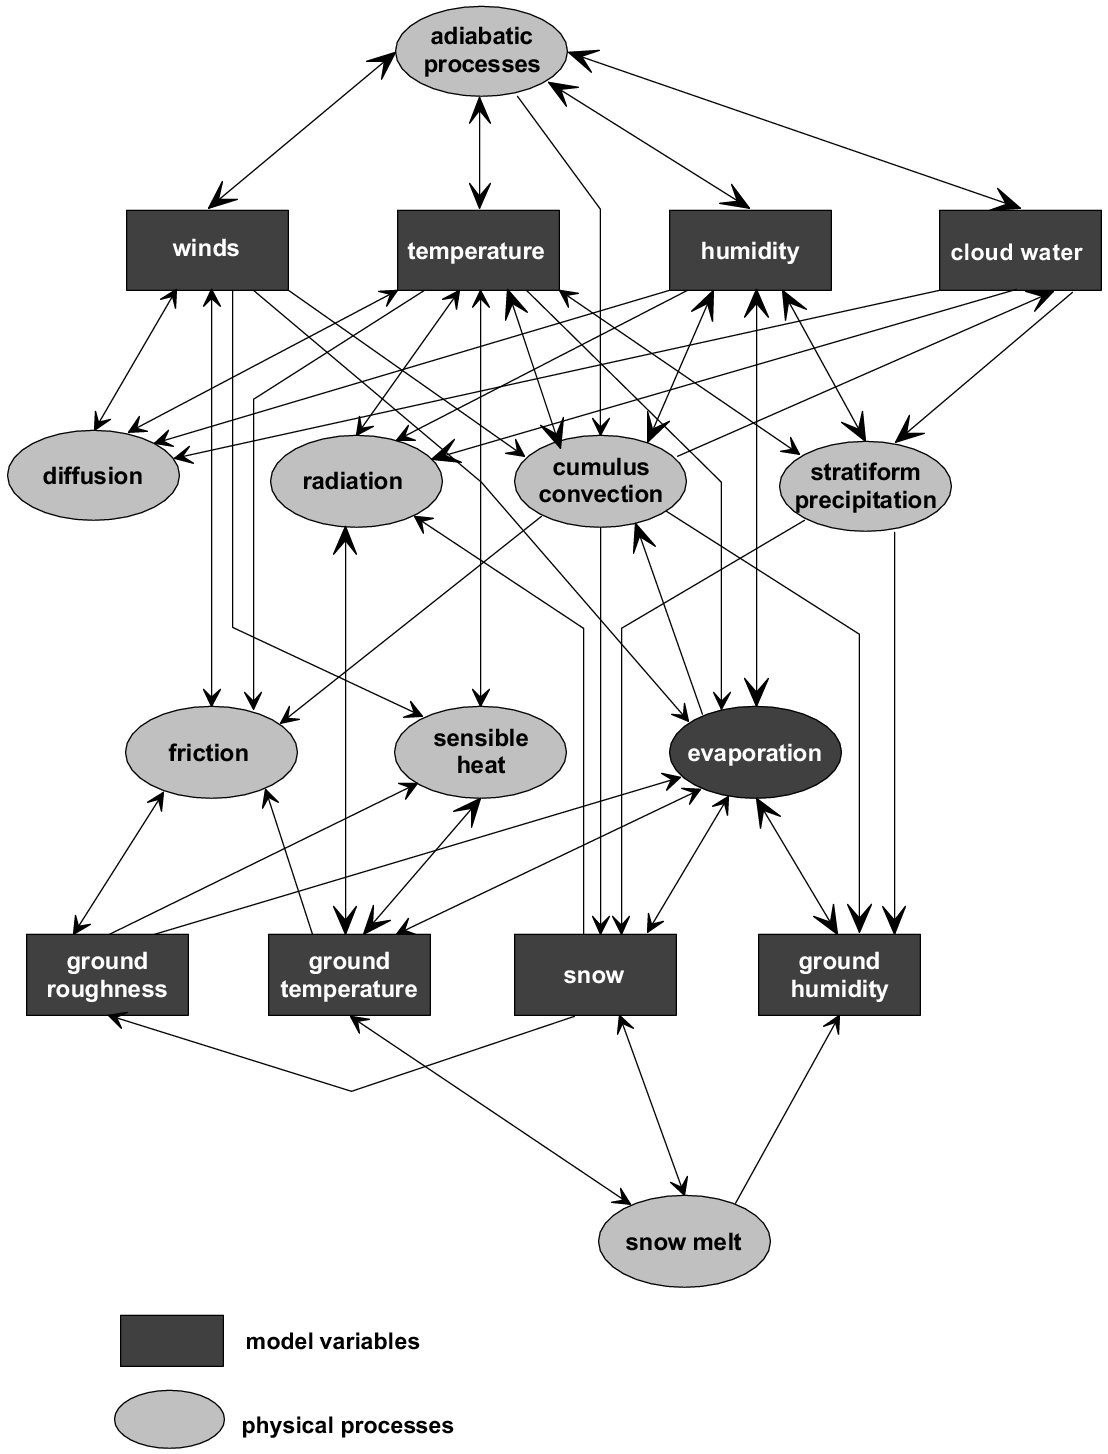
\includegraphics[height=15cm]{Pics/Processes_ECHAM}
%\centering \epsfig{figure=Tr_z.Eng.eps, width=\linewidth}
\end{minipage}
\setlength{\unitlength}{1cm}

\vspace{-2cm}

\begin{minipage}{.5\linewidth}
\begin{picture}(6,8)
\thicklines

\newsavebox{\ovalbox}
\savebox{\ovalbox}(0,0){
   \thicklines
   \put(0,-0.5){\oval(2.0,0.7)}}
\newsavebox{\frbox}
\savebox{\frbox}(0,0){
   \thicklines
   \put(0,-0.5){\framebox(2.0,0.7)}}

\put(4,4.2){\usebox{\ovalbox}}
\put(3.35,3.95){\scriptsize \shortstack[c]{Adiabatic \\ processes}}

\put(4,3.75){\vector(3,-2){1.5}}
\put(5.5,2.75){\vector(-3,2){1.5}}
\put(4,3.75){\vector(-3,-2){1.5}}
\put(2.5,2.75){\vector(3,2){1.5}}

\put(1.5,2.4){\usebox{\frbox}\makebox(2.05,0){\scriptsize Winds}}
\put(4.5,2.4){\usebox{\frbox}\makebox(2.1,0){\scriptsize Temperature}}

\put(2.5,2.05){\vector(0,-1){1.05}}
\put(2.5,1.05){\vector(0,1){1.}}
\put(5.5,2.05){\vector(0,-1){1.05}}
\put(5.5,1.05){\vector(0,1){1.}}

\put(2.5,0.7){\usebox{\ovalbox}}
\put(2.5,0.6){\makebox(0,0){\scriptsize Friction}}
\put(5.5,0.7){\usebox{\ovalbox}}
\put(4.95,0.4){\scriptsize \shortstack[c]{Diabatic \\ heating}}

\end{picture}
\end{minipage}

\vspace{1cm}

\caption{Processes in ECHAM (a) and PUMA (b)}
\label{ProcessesFig}
\end{figure}

\section{Scientific applications}
     The PUMA code is the dynamical core of a GCM forced by Newtonian
     cooling and Rayleigh friction, such as that proposed by Held \&
     Suarez (1994) to evaluate the dynamical cores of GCMs. It forms
     the basis for various applications:
\begin{itemize}
   \item The code can be utilized
     to build and test new numerical algorithms (like semi-Langrangian
     techniques).
   \item Idealized experiments can be performed to analyze nonlinear
     processes arising from internal atmospheric systems (life cycles,
     etc.).
   \item Data assimilation techniques can be incorporated to
     interpret results from GCM simulations or observations.
\end{itemize}

    Figure \ref{ProcessesFig} (a) demonstrates the complexity of the 
    interactions in a full size climate model, which leads to similar 
    complex response patterns from small parameter changes. The same 
    diagram for PUMA Figure \ref{ProcessesFig} (b) shows the simple 
    and direct paths which allow the easy identification of the effects 
    from changes to this model.

\section{Requirements}
   PUMA is open source, everyone may download and use it.
   Though it's easy to use,
   the design of experiments and the interpretation of the results
   require a thorough knowledge of atmospheric science.

   PUMA is available as FORTRAN-90 source code. So all that is needed
   to use PUMA on any computer is a FORTRAN-90 compiler.
   The GUI additionally requires a C-compiler with the graphical
   library X11, which is standard on any UNIX/Linux system
   as well as on newer MACs.
   Windows user may try a X11-emulator like Cygwin.

   The program was developed and tested with several operating systems
   including LINUX, MAC-OS, and Solaris. The main development was done
   using Linux and MAC-OS and the FORTRAN compiler gfortran and sunf90.

   The postprocessor Pumaburner requires a C++ compiler.

   There are several compilers available for the Linux operating system.
   MoSt, PUMA, and Planet Simulator were successfully tested with:

\begin{itemize}
\item SunStudio12 (development environment including
   FORTRAN-90, C, C++, and Debugger) for Solaris and Linux.
   SunStudio12 can be downloaded for free from {\url{http://www.sun.com}}.
\item Gnu FORTRAN (gfortran).
   This free and open access FORTRAN-90 compiler is part of most
   Linux distributions.
   It's also available from
   {\url{http://directory.fsf.org/devel/compilers/gfortran.html}}.
\end{itemize}




\section{History}
    
    The University of Hamburg PUMA model originates from
     the Hoskins \& Simmons SGCM ({\bf S}imple {\bf G}eneral {\bf C}irculation {\bf M}odel)
     version (\citep{hossim75}). The major differences between PUMA
     and its predecessor SGCM are:

\begin{itemize}
   \item The code is rewritten in portable
     FORTRAN-90 code, which removes problems associated with
     machine-specific properties like word lengths, floating point
     precision, output, etc. All the necessary routines are
     in the source code including the
     FFT ({\bf F}ast {\bf F}ourier {\bf T}ransformation)
     and the Legendre Transformation. The model can be run
     on any computer with a standard FORTRAN-90 compiler.
     The MPI-library is needed to run
     PUMA on parallel machines (see below).
     The Xlib (X11R6) library is needed for the graphical user
     interface.
   \item  The
     truncation scheme is changed from the jagged triangular truncation
     to the standard triangular truncation scheme making it compatible to other
     T-models like ECHAM.

   \item  The PUMA/Pumaburner system is data compatible to ECHAM/Afterburner.
     Thus all other ECHAM diagnostic software can be used on PUMA data.

   \item PUMA is fully parallelized and can use as many CPU's 
    as half of the number of latitudes (e.g. 16 in T21 resolution). It uses the MPI
    ({\bf M}essage {\bf P}assing {\bf I}nterface) library while
    running on parallel systems or a cluster.
    MPI is not needed for running PUMA on a single CPU.

   \item  The ongoing development added several new features like the preprocessor,
   graphical user interface, spherical harmonics mode selection, and many more.

\end{itemize}
